%% sfc.tex — PORTER: a plan-committed router for distributed quantum computers
%% Compile:
%%   pdflatex sfc
%%   bibtex   sfc
%%   pdflatex sfc
%%   pdflatex sfc

\documentclass[journal]{IEEEtran}
\IEEEoverridecommandlockouts

\usepackage{cite}
\usepackage{amsmath,amssymb,amsfonts}
\usepackage{algorithmic}
\usepackage{algorithm}
\usepackage{graphicx}
\usepackage{textcomp}
\usepackage{xcolor}
\usepackage{booktabs}
\usepackage{enumitem}
\usepackage{multirow}
\usepackage{url}
\usepackage{tikz}
\usepackage{pgfplots}
\pgfplotsset{compat=1.18}
\usetikzlibrary{shapes.geometric,arrows,arrows.meta,positioning,fit,backgrounds,patterns,decorations.pathmorphing,calc}

%% ── Figure styles ────────────────────────────────────────────────────────────
\tikzset{
  slot/.style={circle,draw=black!60,fill=white,inner sep=0pt,minimum size=7pt},
  occ/.style={slot,fill=black!25},
  portslot/.style={rectangle,draw=black!60,fill=white,inner sep=0pt,minimum size=7.5pt},
  bigslot/.style={slot,minimum size=12pt,font=\tiny},
  bigocc/.style={bigslot,fill=black!15},
  bigport/.style={portslot,minimum size=12.5pt,font=\tiny},
  dagnode/.style={circle,draw,inner sep=1pt,minimum size=14pt,font=\scriptsize},
  dagfront/.style={dagnode,fill=blue!15,thick},
  dagedge/.style={-{Stealth[length=1.6mm]},semithick},
  flowbox/.style={rectangle,rounded corners=2pt,draw,align=center,
                  font=\scriptsize,inner sep=3pt},
  flowdec/.style={diamond,aspect=2.4,draw,align=center,font=\scriptsize,
                  inner sep=0.5pt},
  flowarr/.style={-{Stealth[length=2mm]},semithick},
  eprlink/.style={decorate,decoration={snake,amplitude=.5mm,segment length=1.8mm},
                  red!70!black,semithick},
  catline/.style={densely dashed,blue!60!black,semithick},
}
\usepackage[colorlinks=true,linkcolor=blue,citecolor=blue,urlcolor=blue]{hyperref}

\def\BibTeX{{\rm B\kern-.05em{\sc i\kern-.025em b}\kern-.08em
    T\kern-.1667em\lower.7ex\hbox{E}\kern-.125emX}}

%% ── Notation macros ─────────────────────────────────────────────────────────
\newcommand{\PORTER}{\textsc{PORTER}}
\newcommand{\TeleSABRE}{\textsc{TeleSABRE}}
\newcommand{\dSABRE}{\textsc{dSABRE}}
\newcommand{\SABRE}{\textsc{SABRE}}
\newcommand{\LightSABRE}{\textsc{LightSABRE}}
\newcommand{\TeleData}{\textsc{TeleData}}
\newcommand{\TeleGate}{\textsc{TeleGate}}
\newcommand{\TeleGatePacket}{\textsc{TeleGatePacket}}
\newcommand{\arch}{\mathcal{A}}
\newcommand{\dL}{d_{\mathrm{L}}}
\newcommand{\dC}{d_{\mathrm{C}}}
\newcommand{\logi}[1]{\mathrm{q}_{#1}}
\newcommand{\phys}[1]{\mathrm{p}_{#1}}

%% ── Appendix references ─────────────────────────────────────────────────────
%% Appendices A–D live in the standalone supplement sfc_appendix.tex; the
%% letters below are hardcoded and must match its section order.
\newcommand{\appSuite}{Appendix~A}
\newcommand{\appPytket}{Appendix~B}
\newcommand{\appOptin}{Appendix~C}
\newcommand{\appVerification}{Appendix~D}
\newcommand{\appCatent}{Appendix~E}
\newcommand{\appExample}{Appendix~F}
\newcommand{\appMix}{Appendix~G}
\newcommand{\appTables}{Appendix~H}

\begin{document}

\title{PORTER: A Plan-Committed Router for Multi-Core Distributed Quantum Computers}

\author{Fuchao~Sheng, Yongjian Xie, Yongming Li, Sanjiang~Li~\IEEEauthorrefmark{1}%
\thanks{F. Sheng, Y. Xing, and Y. Li are with the School of Mathematics and Statistics, Shaanxi Normal University, Xi'an, China; S. Li is with the Centre for Quantum Software and Information,
  University of Technology Sydney, Australia
  (e-mail: sanjiang.li@uts.edu.au).}%
\thanks{\IEEEauthorrefmark{1}ORCID: 0000-0002-3332-2546.}}

\maketitle

%%────────────────────────────────────────────────────────────────────────────
\begin{abstract}
A distributed quantum computer runs one circuit across several small
cores joined by links that distribute entanglement on demand, and the
compiler's figure of merit is how few Einstein--Podolsky--Rosen (EPR)
pairs it spends on gates that straddle cores. We present \PORTER{}, a
compiler for such machines. It unifies the three known inter-core
primitives --- state teleportation, gate teleportation and multi-gate
cat-entangler packets --- under one \emph{plan-committed} decision loop
that chooses a complete inter-core action before generating the SWAPs
that make it executable; adds a two-tier capacity-relief mechanism that
routes qubits toward reservoir cores when every candidate is blocked;
and builds its initial layout with a deterministic, seed-free
\emph{temporal locality-greedy} heuristic in place of a seeded search.
On MQT-Bench suites at 25, 64 and 80 logical qubits a single \PORTER{}
pass lowers geometric-mean EPR consumption against published
\TeleSABRE{} by $59.6\%$, $35.8\%$ and $61.3\%$, and completes all
twenty-four instances including seven on which \TeleSABRE{} does not
converge. Against \dSABRE{}, a concurrent compiler revised during this
work and therefore re-run rather than quoted, \PORTER{} is competitive:
$1.05\times$ its pooled EPR at $0.74\times$ its compile time under each
compiler's own protocol, \emph{ahead} of it on forty-one identical
externally supplied layouts and on both heavy-hex core graphs, and
$1.24\times$ behind on a $100$--$360$-qubit scale-up suite. A
controlled ablation then isolates what each design decision buys, and
two of them do not buy EPR pairs --- which we report as measured. Every
run is certified by an independent replay verifier; the
implementation, verifier and harness are public.
\end{abstract}

\begin{IEEEkeywords}
distributed quantum computing, quantum circuit compilation,
multi-core quantum architectures, gate teleportation, cat-entangler packets,
plan-committed routing, entanglement cost
\end{IEEEkeywords}

%%────────────────────────────────────────────────────────────────────────────
\section{Introduction}
\label{sec:intro}

A distributed quantum computer (DQC) runs one circuit across several small
quantum processing units --- \emph{cores} --- joined by links that
distribute entanglement on demand~\cite{cuomo2020towards,escofet2024review}.
What such a machine is short of is not gates but entanglement. Any two-qubit
gate whose operands sit in different cores has to be bought with
Einstein--Podolsky--Rosen (EPR) pairs, and on current hardware distributing
a pair is far slower and far less reliable than any operation performed
inside a core~\cite{stephenson2020high,daiss2021quantum}. How few pairs a
compiler spends is therefore the figure of merit that matters.

There is more than one way to spend a pair. A \emph{state} can be
teleported (\TeleData{}), relocating a logical qubit so every later
gate it meets in its new core is free~\cite{bennett1993teleporting}. A
\emph{gate} can be teleported (\TeleGate{}) through a cat-entangler,
executing one remote CX with neither operand
moving~\cite{eisert2000optimal,yimsiriwattana2004generalized}. Or one
cat-entangled resource can be held open across a run of remote CX gates
sharing a control, so the run costs one pair instead of one each --- a
\emph{packet}, in the spirit of AutoComm's gate-sequence
amortisation~\cite{wu2022autocomm}. They differ in exactly one respect
that matters: how many gates a pair is spread over, which is a property
of the circuit structure where the primitive is applied and not of the
primitive itself, so none of the three dominates.

The choice must be made before its price is known. Each alternative
becomes executable only after its own preparation --- the right operand
beside the right communication port, that port free, the destination
holding a spare slot --- and preparation is work the compiler will not
perform unless it selects that alternative. Scoring an action together
with the preparation it currently needs therefore ranks candidates by
the layout the compiler happens to be sitting in rather than by the
progress they buy, and staging a losing candidate still perturbs the
layout, so effort is spent preparing actions never taken.

\PORTER{} --- a \emph{Plan-Oriented Router for Teleportation-Enabled
aRchitectures} --- keeps the two questions apart. Its unit of choice is
a \emph{plan}: a complete, committable specification of one inter-core
action --- which primitive fires, which gate or same-control run it
resolves, in which direction, and hence which readiness conditions it
needs --- with the SWAP sequence that would establish those conditions
deliberately left out. Whole plans are compared on the gate progress
they buy; one is committed; only then are preparation SWAPs generated,
for that plan alone. Around this loop \PORTER{} adds a two-tier
capacity-relief mechanism that manufactures free slots when every
candidate is capacity-blocked, and a deterministic, seed-free initial
layout replacing the seeded best-of-$N$ search its predecessors run.

\textbf{Results.} We evaluate on MQT-Bench~\cite{quetschlich2023mqtbench}
suites at 25, 64 and 80 logical qubits, on a $100$--$360$-qubit
scale-up series, and on two networks of IBM heavy-hex cores --- forty-eight
circuit--architecture instances. Against
\TeleSABRE{}~\cite{russo2025telesabre}, the published state of the art
for this cost model, \PORTER{} is decisively better: a single pass
lowers geometric-mean EPR consumption by $59.6\%$, $35.8\%$ and
$61.3\%$ on the three suites, and it completes every instance,
including the seven --- among them an 80-qubit, $23{,}381$-CX circuit
--- on which \TeleSABRE{} does not converge in three seeds.

The second comparison is less one-sided and we report it in full.
\dSABRE{}~\cite{lidsabre} is concurrent work on the same problem whose
router was substantially revised while this paper was in preparation,
so we re-ran it from source rather than quoting its tables. Against
that version \PORTER{} is \emph{competitive rather than dominant}.
Under each compiler's own protocol one \PORTER{} pass costs
$1.19\times$ \dSABRE{}'s pooled geometric-mean EPR; restoring a
comparable pass budget reaches $1.05\times$ at $0.74\times$ its compile
time. Routed from identical externally supplied layouts at matched pass
budgets \PORTER{} moves \emph{ahead} across forty-one instances
($126.6$ against $134.2$), and on both heavy-hex core graphs it takes
the suite. On the $100$--$360$-qubit series it trails by $1.24\times$
even with the layout controlled. The two compilers share four
load-bearing design decisions, set out in Section~\ref{sec:related} so
that neither is credited with the other's.

\textbf{What the mechanisms are worth.} Because the two compilers are
close relatives, a head-to-head number says little about which design
decision earns its place, so we ablate each of \PORTER{}'s in isolation
and report the outcome as measured rather than as advertised. Two of
the four answers are negative. Capacity relief is what makes a
deterministic-greedy design complete at all --- without it four of six
80-qubit instances deadlock --- and the initial layout is what
separates the two compilers below roughly a hundred physical qubits.
But plan commitment reaches the same EPR as re-scoring the whole front
every iteration, within $0.6\%$ and on the same number of routing
moves, so what it buys is $1.3$--$3\times$ less compile time rather
than better routes. And the packet primitive, which exists to amortise
a pair across a run of gates, is \emph{outperformed at 80 qubits by
removing gate teleportation altogether}, by $32.8\%$.

\textbf{Contributions.} We contribute \PORTER{} itself --- a
deterministic, seed-free DQC compiler that routes in a single forward
pass, built around the plan-first remote stage of
Section~\ref{sec:sfc-plan-first}, the two-tier capacity relief of
Section~\ref{sec:sfc-relief}, and the temporal locality-greedy layout
of Section~\ref{sec:sfc-layout}, with an optional refinement schedule
that trades compile time back for EPR pairs. We contribute an
evaluation across forty-eight circuit--architecture instances --- under
each compiler's own protocol, under shared fixed layouts, with each
compiler routing the other's layout, and on two heavy-hex core graphs
--- in which \PORTER{} beats published \TeleSABRE{} decisively and is
competitive with concurrent \dSABRE{}, and every reported run is
certified by an independent replay verifier that re-derives gate
coverage, dependency order and physical legality from the emitted
operation stream alone. And we contribute an ablation that decides what
to believe about each mechanism (Section~\ref{sec:ablation}), including
the two answers that are negative.

The \PORTER{} implementation, the replay verifier, the full cross-router
comparison harness, and the raw per-circuit results are publicly available at
\url{https://github.com/ebony72/porter}.

%%────────────────────────────────────────────────────────────────────────────
\section{Background}
\label{sec:background}

\subsection{Quantum Circuits and Routing}
\label{sec:qcircuits}

A circuit acts on $n$ logical qubits through a sequence of gates; we
work in the restricted basis $\{\texttt{id}, \texttt{rz}, \texttt{sx},
\texttt{x}, \texttt{cx}\}$ of MQT-Bench's Qiskit-opt3-transpiled
circuits~\cite{quetschlich2023mqtbench}, i.e.\ arbitrary one-qubit
gates plus the two-qubit CX. A circuit is a directed acyclic graph
(DAG): for every logical qubit, consecutive gates acting on it are
joined by a dependency edge. The \emph{front} is the set of gates with
no unexecuted predecessor; only front gates can execute or be routed
towards execution. Gates sharing a qubit --- two CX gates with the same
control, say --- are chained by a dependency edge and therefore
\emph{never} appear in the front together, a fact that matters for
packet collection (Section~\ref{sec:sfc-packet}).

Physical qubits are partitioned into \emph{cores}; each core has an
intra-core coupling graph, and pairs of cores may be joined by an
inter-core link whose two endpoints are designated \emph{communication
ports}. A \emph{layout} maps every logical qubit to a physical
position. A two-qubit gate is \emph{local} if both operands share a
core and \emph{remote} otherwise; routing a local gate that is not yet
adjacent requires intra-core SWAPs, and routing a remote gate requires
an inter-core communication primitive. We write $\kappa_\ell(q)$ for
the core holding $q$ under layout $\ell$, $\dL(c,p,p')$ for
intra-core distance and $\dC(c,c')$ for core-graph distance.

\subsection{Communication Primitives}
\label{sec:primitives}

Three inter-core primitives are in play, sketched in
Figure~\ref{fig:primitives}; each consumes exactly one EPR pair.

\begin{figure}[t]
\centering
% ---- (a) TeleData ----
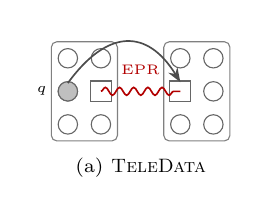
\begin{tikzpicture}[x=0.42cm,y=0.42cm]
  % left core (2x3), port = right-middle; right core, port = left-middle
  \foreach \ox in {0,3.4}{
    \draw[rounded corners=2pt,black!50] (\ox-0.5,0.5) rectangle (\ox+1.5,-2.5);
    \foreach \xx in {0,1} \foreach \yy in {0,1,2}
      \node[slot] at (\ox+\xx,-\yy) {};
  }
  \node[portslot] at (1,-1) {};
  \node[portslot] at (3.4,-1) {};
  \draw[eprlink] (1,-1) -- (3.4,-1);
  \node[font=\tiny,red!70!black] at (2.2,-0.35) {EPR};
  \node[occ] at (0,-1) {};
  \node[font=\tiny,anchor=east] at (-0.35,-1) {$q$};
  \draw[-{Stealth[length=1.8mm]},semithick,black!70]
    (0,-0.75) .. controls (1.2,0.9) and (2.4,0.9) .. (3.4,-0.72);
  \node[font=\scriptsize] at (2.2,-3.3) {(a) \TeleData};
\end{tikzpicture}\hfill
% ---- (b) TeleGate ----
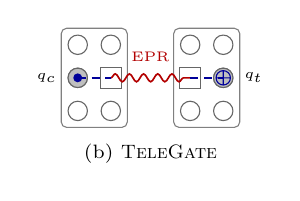
\begin{tikzpicture}[x=0.42cm,y=0.42cm]
  \foreach \ox in {0,3.4}{
    \draw[rounded corners=2pt,black!50] (\ox-0.5,0.5) rectangle (\ox+1.5,-2.5);
    \foreach \xx in {0,1} \foreach \yy in {0,1,2}
      \node[slot] at (\ox+\xx,-\yy) {};
  }
  \node[portslot] at (1,-1) {};
  \node[portslot] at (3.4,-1) {};
  \draw[eprlink] (1,-1) -- (3.4,-1);
  \node[font=\tiny,red!70!black] at (2.2,-0.35) {EPR};
  \node[occ] at (0,-1) {};
  \node[occ] at (4.4,-1) {};
  \node[font=\tiny,anchor=east] at (-0.35,-1) {$q_c$};
  \node[font=\tiny,anchor=west] at (4.75,-1) {$q_t$};
  \draw[catline] (0,-1) -- (1,-1);
  \draw[catline] (3.4,-1) -- (4.4,-1);
  \filldraw[blue!60!black] (0,-1) circle (1.4pt);
  \draw[blue!60!black] (4.4,-1) circle (2.6pt)
    +(0,-2.6pt) -- +(0,2.6pt) +(-2.6pt,0) -- +(2.6pt,0);
  \node[font=\scriptsize] at (2.2,-3.3) {(b) \TeleGate};
\end{tikzpicture}\hfill
% ---- (c) TeleGatePacket ----
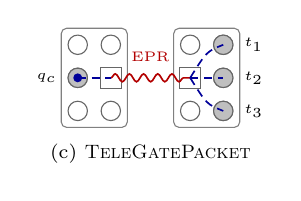
\begin{tikzpicture}[x=0.42cm,y=0.42cm]
  \foreach \ox in {0,3.4}{
    \draw[rounded corners=2pt,black!50] (\ox-0.5,0.5) rectangle (\ox+1.5,-2.5);
    \foreach \xx in {0,1} \foreach \yy in {0,1,2}
      \node[slot] at (\ox+\xx,-\yy) {};
  }
  \node[portslot] at (1,-1) {};
  \node[portslot] at (3.4,-1) {};
  \draw[eprlink] (1,-1) -- (3.4,-1);
  \node[font=\tiny,red!70!black] at (2.2,-0.35) {EPR};
  \node[occ] at (0,-1) {};
  \node[font=\tiny,anchor=east] at (-0.35,-1) {$q_c$};
  \node[occ] at (4.4,0) {};
  \node[occ] at (4.4,-1) {};
  \node[occ] at (4.4,-2) {};
  \node[font=\tiny,anchor=west] at (4.75,0) {$t_1$};
  \node[font=\tiny,anchor=west] at (4.75,-1) {$t_2$};
  \node[font=\tiny,anchor=west] at (4.75,-2) {$t_3$};
  \draw[catline] (0,-1) -- (1,-1);
  \filldraw[blue!60!black] (0,-1) circle (1.4pt);
  \draw[catline] (3.4,-1) .. controls (3.9,-0.2) .. (4.4,0);
  \draw[catline] (3.4,-1) -- (4.4,-1);
  \draw[catline] (3.4,-1) .. controls (3.9,-1.8) .. (4.4,-2);
  \node[font=\scriptsize] at (2.2,-3.3) {(c) \TeleGatePacket};
\end{tikzpicture}
\caption{The three communication primitives; each consumes one EPR
  pair between the two communication ports (squares). (a)~\TeleData{}
  moves qubit $q$ (which must sit adjacent to its free port) onto the
  free destination port. (b)~\TeleGate{} executes one remote CX
  through a cat-entangler~\cite{yimsiriwattana2004generalized}
  (\appCatent{}): the target-side port acts as a proxy for
  the control $q_c$; neither qubit moves. (c)~\TeleGatePacket{}
  brackets an ordered run of remote CX gates sharing the control $q_c$
  between one cat-entangler/disentangler pair, amortising a single
  EPR pair over the whole run; each target is routed next to the port
  in turn while the ports stay reserved.}
\label{fig:primitives}
\end{figure}

\textbf{State teleportation (\TeleData{}).} Consumes one EPR pair to
move a logical qubit from a communication port in one core to a free
port in another, after which every later gate that qubit meets in its
new core is local. Its value is therefore \emph{latent}: it is paid
once and repaid over however many future gates the relocation makes
local.

\textbf{Gate teleportation (\TeleGate{}).} Executes a single remote CX
with neither operand moving. One EPR pair entangles the two
communication ports; a \emph{cat-entangler} ---
$\mathrm{CX}(q_c,e_A)$, measurement of $e_A$, and a classically
controlled $X$ on $e_B$ --- leaves $(q_c,e_B)$ in the cat state
$\alpha|00\rangle + \beta|11\rangle$, so every CX controlled by the
remote port $e_B$ acts as if controlled by $q_c$. A
\emph{cat-disentangler} --- Hadamard on $e_B$, measurement, a
classically controlled $Z$ on $q_c$ --- restores $q_c$ and frees both
ports (\appCatent{}). Its value is entirely \emph{direct}: exactly one
gate, and nothing is left behind.

\textbf{Same-control packets (\TeleGatePacket{}).} When several remote
CX gates share the same control and their targets lie in one core, the
run can be bracketed between a \emph{single} cat-entangler and
disentangler: the ports stay reserved, each target is routed beside
$e_B$ in turn, and the whole run costs one EPR pair instead of one
each. This is the amortisation idea of AutoComm~\cite{wu2022autocomm},
specialised to the shared-control case and applied inside a routing
loop rather than as a pre-pass. Because same-control gates are chained
by DAG dependency edges they never appear in the front together, so a
packet cannot be read off the front and has to be collected by forward
simulation (Section~\ref{sec:sfc-packet}).

The three differ in exactly one respect that matters for scoring: how
many gates one pair is spread over. \TeleData{} amortises over an
unknown future, \TeleGate{} over exactly one gate, and
\TeleGatePacket{} over a run whose length the compiler must discover.
Section~\ref{sec:sfc-scoring} makes that difference explicit as a
direct/latent/lookahead decomposition, and Section~\ref{sec:ablation}
measures whether the richer vocabulary is worth having.

\subsection{SABRE}
\label{sec:sabre}

\SABRE{}~\cite{li2019tackling} routes a single-core circuit by
repeatedly selecting the SWAP that minimises a front-layer distance
term plus a weighted extended-set lookahead term, both expressed as
$\Delta$ (old distance minus new distance) on gates sharing a qubit
with the candidate SWAP. \PORTER{} inherits this scoring form for its
intra-core stage (Section~\ref{sec:sfc-intra}) and extends the same
direct/lookahead decomposition to its inter-core plan scorer
(Section~\ref{sec:sfc-scoring}).

%%────────────────────────────────────────────────────────────────────────────
\section{The \PORTER{} Compiler}
\label{sec:sfc}

Given a circuit and an initial layout $\ell_0$ (which \PORTER{} builds
itself, Section~\ref{sec:sfc-layout}), \PORTER{} repeats the following
loop (Algorithm~\ref{alg:sfc}) until every gate has been emitted or a
configurable iteration budget is exhausted. Algorithm~\ref{alg:sfc}
charts one iteration; its shaded region is the plan-first remote stage
that distinguishes \PORTER{} from compilers deciding at
single-action granularity; \appExample{} walks through it on a concrete
front where it changes the outcome.


\begin{algorithm}[t]
\caption{\PORTER{} \texttt{compile}$(C, \ell_0)$}
\label{alg:sfc}
\begin{algorithmic}[1]
\STATE $\ell \leftarrow \ell_0$; initialise DAG active/frontier sets from $C$
\WHILE{DAG has active gates}
  \STATE $F \leftarrow$ DAG front (bounded by \texttt{dag\_front\_limit})
  \STATE classify $F$ into singles, direct-local CX, local-CX-needing-SWAP,
         adjacent-remote CX, non-adjacent-remote CX \hfill\textit{(Sec.~\ref{sec:sfc-classify})}
  \IF{singles or direct-local CX present}
    \STATE execute them all; remove from DAG; \textbf{continue}
  \ENDIF
  \IF{local-CX-needing-SWAP present}
    \STATE generate candidate intra-core SWAPs, apply the best-scoring one
           (Eq.~\ref{eq:sfc-local}); \textbf{continue} \hfill\textit{(Sec.~\ref{sec:sfc-intra})}
  \ENDIF
  \STATE generate normal remote plans $\mathcal{P}$ and blocked-teleport
         plans $\mathcal{B}$ \hfill\textit{(Sec.~\ref{sec:sfc-scoring})}
  \IF{$\mathcal{P}\neq\emptyset$}
    \STATE $p^\ast \leftarrow$ best ready-or-preparable plan in $\mathcal{P}$
    \IF{some $b\in\mathcal{B}$ has gain $\gg$ gain$(p^\ast)$}
      \STATE $p^\ast \leftarrow$ best opportunistic capacity-relief plan for $b$
             \hfill\textit{(Sec.~\ref{sec:sfc-relief})}
    \ENDIF
  \ELSE
    \STATE BFS from each blocked target core to its nearest reservoir;
           $p^\ast \leftarrow$ best tail-relief plan \hfill\textit{(Sec.~\ref{sec:sfc-relief})}
  \ENDIF
  \IF{$p^\ast$ is \texttt{None}} \STATE \textbf{report deadlock; abort} \ENDIF
  \STATE apply $p^\ast$'s own preparation SWAPs until ready, then execute it
\ENDWHILE
\RETURN emitted operations, final layout, stats
\end{algorithmic}
\end{algorithm}

\subsection{Initial Layout}
\label{sec:sfc-layout}

\PORTER{} builds its starting layout $\ell_0$ with one deterministic,
seed-free heuristic --- no external partitioner, no best-of-$N$ search
--- and respects the capacity invariant the routing loop depends on:
every core keeps at least $f_\mathrm{min}{=}2$ free positions, so from
the first iteration any core can serve as a \TeleData{} destination and
as a relief reservoir.

\textbf{Temporal locality-greedy.} Three deterministic steps.
\emph{(i) Weighting}: each CX gate $g=(q_i,q_j)$ contributes
$\gamma^{\ell(g)}$ to the interaction weight $w(q_i,q_j)$, where
$\ell(g)$ is $g$'s as-soon-as-possible layer in the CX-only DAG and
$\gamma{=}0.99$, so early interactions weigh more than late ones while
repeated interactions accumulate. \emph{(ii) Core assignment}: logical
qubits are visited in the order they first appear as a CX operand and
each is placed in the core holding its heaviest already-placed
neighbour when that core has headroom above $f_\mathrm{min}$, falling
back to the core with the most remaining reserved capacity.
\emph{(iii) Physical placement}: within each core, logicals are laid
onto positions by descending interaction weight onto ascending
intra-core centrality, so the most-connected qubits take the most
central slots.

The steps are complementary. The temporal discount front-loads the
opening layers, co-locating the pairs that must interact soonest;
accumulated multiplicity plus first-appearance order tracks
chain-structured circuits, where only one disjoint pair is exposed per
layer and a balanced-first-layer rule would scatter the chain across
cores; and the centrality step keeps hub qubits cheap to reach. The
construction costs microseconds and consumes no randomness, so
\PORTER{} has no seed to report.

\subsection{Backward Refinement}
\label{sec:sfc-refine}

\PORTER{}'s default protocol is one forward pass from $\ell_0$. We also
report an optional refinement schedule, because
Section~\ref{sec:shared_results} shows a fixed layout is not the whole
difference between the two compilers: given the \emph{same} externally
supplied layout, \dSABRE{}'s forward--backward--forward schedule
extracts more from it than a single forward pass does.

The schedule is \SABRE{}'s bidirectional layout
refinement~\cite{li2019tackling} applied to whole routes. Let $R(C,\ell)$
denote routing $C$ from $\ell$ and $\ell'$ the layout it ends on.
Pass~1 computes $R(C,\ell_0)$; pass~2 computes
$R(C^{\mathrm{rev}},\ell_1')$ on the reversed circuit and
\emph{discards its route}, keeping only $\ell_2'$; pass~3 computes
$R(C,\ell_2')$. Reversing $C$ reverses every dependency edge, so
routing it from the forward pass's end state yields a layout adapted to
the \emph{start} of the forward circuit. Odd pass counts above three
repeat the cycle; $P{=}5$ throughout. We report the best forward pass
by EPR, so refinement can never report worse than the single pass. It
adds no randomness and its whole cost is routing passes --- $P$ calls
where the default makes one, against \dSABRE{}'s nine.

It recovers less here than it does for \dSABRE{}, and the reason is
instructive. Refinement consumes a post-routing layout, and routing
destroys the structure $\ell_0$ was built with: on 64-qubit AE $\ell_0$
leaves $(2,2,2,2,8,16)$ free slots per core --- packed cores plus two
reservoirs, exactly the shape the capacity machinery wants --- and one
forward pass scrambles that to $(14,1,12,2,1,2)$. Intermediate passes
therefore often regress (64q~AE $177 \to 308$, 64q~QFT $262 \to 326$),
which only the best-pass rule keeps harmless. Where it pays it pays
well: 64q~QNN $864 \to 537$, 64q~Multiplier $1{,}358 \to 763$.

\subsection{Front Classification}
\label{sec:sfc-classify}

Every front gate is classified under the current layout $\ell$. 1Q
gates are always directly executable; a CX $g=(q_i,q_j)$ with both
operands in core $c$ is \emph{direct-local} if
$\dL(c,\ell(q_i),\ell(q_j))=1$ and \emph{local-needing-SWAP}
otherwise; a CX whose operands lie in different cores is
\emph{adjacent-remote} if those cores are core-graph neighbours and
\emph{non-adjacent-remote} otherwise. Directly executable gates drain
first and completely, intra-core SWAPs are exhausted next, and
remote-stage decisions are taken only once no front gate is
intra-core. The front is size-capped at $96$ gates to bound
per-iteration cost, a cap that never binds here since front gates are
pairwise qubit-disjoint.

\subsection{Intra-Core SWAP Scoring}
\label{sec:sfc-intra}

For a local-needing-SWAP gate set $F_\mathrm{loc}$, \PORTER{} builds
candidate SWAP edges from the coupling-graph neighbours of every
physical position touched by $F_\mathrm{loc}$, simulates each SWAP,
and scores it with \SABRE{}'s front-plus-lookahead
form~\cite{li2019tackling}:
\begin{equation}
  J(a) = \bar d_{\mathcal{F}}(a) + \lambda_\mathrm{loc}\,\bar d_{\mathcal{E}}(a),
  \qquad \lambda_\mathrm{loc}=0.8,
  \label{eq:sfc-local}
\end{equation}
where $\bar d_{\mathcal{F}}(a)$ is the mean, over the gates
$(q_i,q_j)\in F_\mathrm{loc}$, of the intra-core distance
$\dL\bigl(c,\ell_a(q_i),\ell_a(q_j)\bigr)$ under the post-SWAP layout
$\ell_a$, and $\bar d_{\mathcal{E}}(a)$ is the same mean taken over an
extended set $\mathcal{E}_\mathrm{loc}$ of up to
$N_\mathrm{loc}{=}20$ local CX gates collected from the next
$L_\mathrm{loc}{=}12$ DAG layers via a virtual frontier simulation
(Section~\ref{sec:sfc-simstate}). Ties are broken first by the raw
front-layer distance, then, if still tied, by a decision uniformly
sampled from a constant-seeded random-number generator, with every
such tie-break recorded in \texttt{RouterStats} for reproducibility
auditing.

\subsection{Plan-First Remote Stage}
\label{sec:sfc-plan-first}

\PORTER{} manipulates remote work as \emph{plans}. A plan is a
complete, committable specification of one inter-core action: which
primitive fires, which gate or same-control run it resolves, its
direction, and consequently its \emph{readiness conditions} --- which
logical endpoint must sit adjacent to which communication port, and
which ports must be free. What it deliberately leaves unspecified is
the SWAP sequence that establishes those conditions. Alternatives are
compared at the level of \emph{what} remote work to do next, each
scored as if its preconditions were met; only the committed plan is
handed to the machinery that works out \emph{how}.

Both baselines decide at a finer grain. \TeleSABRE{}'s pool holds
staging SWAPs and remote operations together, so the choice is made
implicitly, one micro-move at a time: every staging SWAP it selects is
also a vote for whichever remote action that SWAP happens to serve,
votes for competing actions interleave, and staging effort is routinely
spent on actions never taken. \dSABRE{} does separate the stages, but
its candidate is a single teleport hop rather than a plan, and its
score adds that hop's staging and eviction cost directly to the
progress it buys, so a hop cheap to stage now can outrank one that
resolves more gates. \PORTER{} ranks by gain alone, demotes readiness
cost to a tie-break, and refuses to reopen the choice until the
selected plan is ready (\appExample{}); Section~\ref{sec:ablation}
measures what that persistence is worth.

When the front holds only remote CX gates, \PORTER{} generates two
disjoint candidate sets. \textbf{Normal plans} $\mathcal{P}$: for every
adjacent-remote CX, a \TeleGate{}; a \TeleGatePacket{} if a
same-control run of $\ge 2$ remote CX gates can be collected by
forward DAG simulation (Section~\ref{sec:sfc-packet}); and, for either
endpoint, a \TeleData{} plan into the partner's core if that core has
at least $f_\mathrm{min}{=}2$ free positions. For non-adjacent-remote
CX gates, only distance-reducing \TeleData{} hops with sufficient
destination capacity. \textbf{Blocked plans} $\mathcal{B}$: the same
\TeleData{} candidates for destinations that currently fail the
$f_\mathrm{min}$ test. These are never executed; they exist to detect
when no normal plan exists because every destination is saturated, or
when one is available but a blocked plan promises much more if capacity
were relieved first.

Every plan is scored (Section~\ref{sec:sfc-scoring}) \emph{before} any
preparation SWAP for it exists. \PORTER{} then selects the best plan in
$\mathcal{P}$ that is ready or admits an improving preparation SWAP;
compares its gain against the best of $\mathcal{B}$ and, if the blocked
plan leads by more than $m_\mathrm{assist}{=}5.0$, runs opportunistic
capacity relief for that saturated core instead
(Section~\ref{sec:sfc-relief}); and, if $\mathcal{P}$ is empty, runs
the same breadth-first relief search directly on $\mathcal{B}$'s
destinations, shortest hop count first. Once committed, it generates
and applies \emph{only that plan's} preparation SWAPs until the plan is
ready, no improving SWAP remains, or the full decision state --- plan
identity, layout, RNG state --- repeats, which raises rather than
looping.

\textbf{Preparation SWAPs.}\label{sec:sfc-prep} A committed plan's
readiness requirements are exactly two \emph{(core, neighbour-core,
endpoint)} triples (source and destination side for \TeleData{};
control and target side for \TeleGate{}/\TeleGatePacket{}, whose
target-side routing is deferred to execution time,
Section~\ref{sec:sfc-packet}). For each unmet requirement, candidate
preparation SWAPs are restricted to edges incident to either the
plan's logical endpoint or a nearest free physical position tied for
minimum distance to the relevant communication port (only while that
port remains occupied); each candidate is scored by the post-SWAP
value of the same readiness-cost function used to rank blocked plans
(Section~\ref{sec:sfc-scoring}), and at most one improving SWAP per
core side is applied per pass.

\subsection{Plan Scoring: Direct, Latent, and Lookahead Gain}
\label{sec:sfc-scoring}

Every plan scores $\mathrm{total} = \mathrm{direct} +
\mathrm{lookahead}$, computed per plan kind but sharing one
$\Delta$-form convention: for a CX gate $g=(q_i,q_j)$ and a candidate
relocation, $\Delta(g) = \dC(\kappa(q_i),\kappa(q_j)) -
\dC(\kappa'(q_i),\kappa'(q_j))$, the reduction in core-graph distance
between $g$'s two cores.

A \textbf{\TeleGate{}} contributes a constant direct gain of $1$ --- one
remote CX resolved --- and no lookahead. A \textbf{\TeleGatePacket{}}
contributes a direct gain equal to the number of remote CX gates in the
collected packet; every gate in an accepted packet is current rather
than speculative work, since the whole packet executes under one
cat-entangler resource once started. A \textbf{\TeleData{}} plan
decomposes into three tiers, all computed by simulating the DAG
frontier under the hypothetical post-teleport core assignment:
\emph{direct} --- front-layer CX gates already involving the moving
qubit, plus the seed gate; \emph{latent-direct} --- CX gates on the
moving qubit that surface while the simulator can still progress using
only 1Q and now-local gates, which are current pressure rather than
prediction because the candidate teleport fixes their core distance the
moment they appear; and \emph{lookahead} --- gates on the moving qubit
found in up to $L_\mathrm{tp}{=}16$ further simulated layers (capped at
$N_\mathrm{tp}{=}50$ gates), a gate in layer $k$ entering with weight
$w_k = \max(w_\mathrm{min}, w_0\gamma^{k-1})$, $w_0{=}0.9$,
$\gamma{=}0.9$, $w_\mathrm{min}{=}0.5$. Thus
\begin{align}
  \mathrm{direct} &= \!\!\sum_{g\in\mathrm{direct}\cup\mathrm{latent}}\!\!\Delta(g),
  &
  \mathrm{lookahead} &= \!\!\sum_{(g,k)\in\mathrm{la}}\!\!w_k\,\Delta(g),
  \label{eq:sfc-teleport}
\end{align}
with latent-direct gates entering at full weight alongside direct ones.
A capacity-risk term $1/\max(1,f_\mathrm{dst}{-}1)$ is tracked
alongside the score for tie-breaking, but never added to it.

This is the point at which \PORTER{} differs most sharply from
\dSABRE{}: preparation cost appears nowhere in $\mathrm{total}$. Plans
are ranked on gain, and readiness cost enters only as the third
tie-break in the selection key, after gain and plan kind. Note that
$L_\mathrm{tp}$ and $N_\mathrm{tp}$ are absolute gate counts and do not
scale with the core count --- a design choice
Section~\ref{sec:scaleup} gives reason to revisit.

\subsection{Same-Control Packet Collection}
\label{sec:sfc-packet}

From a seed adjacent-remote CX $g=(q_c,q_t)$ with control core $c_c$
and target core $c_t$, \PORTER{} simulates the DAG frontier forward for
up to $120$ layers, greedily absorbing any front CX sharing control
$q_c$ whose target is also in $c_t$ (up to $8$ such gates) and any
front 1Q gate whose qubit is already in $c_t$, since those execute
freely while the cat resource is live. Collection stops at the first
unproductive layer or at the size cap. The window counts simulated \emph{layers}, not collected CXs, because
same-control CXs are DAG-chained and surface one at a time; in practice
it is a cost guard, not an active knob. Because the simulation admits gates from later
generations than the bounded current front, a packet may contain gates
a naively front-limited scan could not reach. The collected order is
replayed exactly at commit time as one \texttt{cat\_entangler}
(consuming the packet's single pair), one \texttt{cat\_cx} per member
--- each target routed to its port by ordinary local SWAPs forbidden
from touching the two live ports --- and a closing
\texttt{cat\_disentangler}.

\subsection{Capacity Relief}
\label{sec:sfc-relief}

\textbf{Tail-relief BFS.} When every remote plan is capacity-blocked,
\PORTER{} runs a breadth-first search from each blocked destination core
to the nearest \emph{reservoir} core --- one with at least $f_\mathrm{min}$
free slots --- optionally chained beyond one hop
(\texttt{capacity\_relief\_chain\_enabled}). Every logical qubit
currently in the BFS path's penultimate core becomes a tail-relief
\TeleData{} candidate into the reservoir, scored and selected by the
same plan machinery, grouped and tried in ascending hop-count order.

\textbf{Opportunistic relief.} Even when a normal plan is available,
a severely blocked plan can still win if relieving its target core's
capacity would unlock substantially more gain
(Section~\ref{sec:sfc-plan-first}); this differs from tail-relief BFS
in firing pre-emptively, before any plan is actually starved, whenever
the margin $m_\mathrm{assist}$ is exceeded.

\subsection{Progress and the Failure Model}
\label{sec:sfc-progress}

Deterministic greedy routing on a capacity-constrained machine can
stall, and the mechanisms above are best read as one answer to that
risk. \PORTER{} layers four defences.

\emph{(i) Keep capacity from reaching zero.} A core with no free
physical qubit is terminal under the port-based action model: it can
never vacate an occupied communication port with local SWAPs, so no
inter-core action can touch it and its qubits are stranded. \PORTER{}
legalises the entry layout so no core starts full, and admits a
\TeleData{} plan into core $c$ as a \emph{normal} plan only while
$\mathrm{free}(c) \ge f_\mathrm{min}{=}2$. Ordinary routing therefore
cannot drive a core into the terminal state; only an externally
supplied layout can present one, which is why \appPytket{}'s
pytket-dqc source is the only place the compiler reports
\emph{infeasibility}.

\emph{(ii) Detect starvation rather than thrash.} Capacity-blocked
candidates are still generated, into a separate set $\mathcal{B}$. They
are never executed, but an empty plan set alongside a non-empty
$\mathcal{B}$ is an explicit signal that the front is starved \emph{by
capacity}, and it names the cores responsible.

\emph{(iii) Manufacture capacity where it is missing.} Tail-relief BFS
turns that signal into work, evacuating a qubit from the penultimate
core on the path to the nearest reservoir (Section~\ref{sec:sfc-relief}).

\emph{(iv) Bound every loop.} Plan sides whose preparation score is
infinite are never selected; during preparation the compiler hashes its
full decision state --- committed plan, layout, RNG state --- once per
round and raises if it repeats; two budgets bound the loops from
outside; and when no plan can be prepared and no relief path reaches a
reservoir \PORTER{} raises a diagnostic naming the saturated cores.

We state the resulting guarantee precisely, because it is weaker than
it may appear. \PORTER{} is \emph{safe} but not \emph{complete}: it
never emits an invalid or partial circuit and always terminates, but
termination may be by exception, and it has no analogue of
\dSABRE{}'s termination-with-success proof
(Section~\ref{sec:related}). Its completeness is empirical, and
Section~\ref{sec:ablation} measures what buys it: with both relief
tiers active none of the twenty-four instances deadlocks in any
protocol; with both disabled, four of the six 80-qubit instances do.
That record is not unbroken, and the exception is instructive: on the
heavy-hex star of Section~\ref{sec:heavyhex}, Multiplier livelocks in
the intra-core SWAP loop --- capacity never reaches zero, no plan is
starved, the diagnostic never fires, and it is the iteration budget
that ends the run. Supplying a comparable worst-case guarantee is the
clearest piece of future work this design leaves open.

\subsection{Computational Complexity}
\label{sec:sfc-complexity}

Let $N$ be the gate count, $n$ the logical-qubit count, $K$ the core
count and $M$ the per-core physical-qubit count. Distance tables are
precomputed once at construction in $O(KM^2\log M + K^2\log K)$,
matching the two-level Dijkstra decomposition comparable compilers
use~\cite{lidsabre}. Per iteration, classification and draining cost
$O(|F|)$; intra-core SWAP scoring evaluates $O(M)$ candidate edges,
each at $O(|F_\mathrm{loc}| + N_\mathrm{loc})$ over one DAG snapshot
reused across candidates; remote-plan scoring evaluates $O(n)$
candidates at $O(N_\mathrm{tp})$ over the same snapshot. Free-slot
queues are $O(1)$ amortised per layout mutation. Summing over $N$
iterations gives $T_\mathrm{total} = O(N(Mn + KM^2\log M))$ excluding
precomputation, in line with other core-local distributed
compilers~\cite{lidsabre,russo2025telesabre}.

%%────────────────────────────────────────────────────────────────────────────
\section{Experimental Evaluation}
\label{sec:experiments}

\subsection{Implementation and Verification}
\label{sec:perf}

\PORTER{} is implemented in Python and is publicly available together
with the verifier and comparison harness. It is fully deterministic and
takes no seed: heuristic ties resolve through a fixed chain of
deterministic keys and any residual tie through a constant-initialised
generator, so for a fixed circuit and hardware the emitted operation
stream is byte-identical across runs, every residual tie-break is
counted in the emitted statistics, and behaviour preservation across
refactorings is certified by hashing the serialised stream. Compile
time is kept low by incremental data structures --- chiefly the
\texttt{DagFrontierSimulator}\label{sec:sfc-simstate} shared by
extended-set collection and teleport lookahead, a copy-on-write view
over the live DAG that tracks a private overlay of predecessor-count
decrements, so a snapshot costs $O(|\text{frontier}|)$ rather than
$O(|\text{remaining circuit}|)$ and independent virtual simulations can
run from one live state without interfering --- together with
incremental frontier maintenance, cached distance tables, $O(1)$
free-slot accounting, and apply/restore SWAP scoring in place of layout
cloning. These cut wall-clock time by roughly $4\times$ against a
straightforward implementation of the same algorithm, with
byte-identical output.

Every reported run is certified by an independent replay verifier that
treats the compiler as a black box: from the emitted operation stream,
the original circuit and the initial layout alone it re-derives gate
coverage (each gate exactly once), per-qubit dependency order,
coupling-edge legality of every local operation, port rules for every
teleport, telegate and packet, and consistency of every reported
statistic. The verifier is itself tested by fault injection --- ten
classes of mutation applied to passing streams, every mutant rejected
(\appVerification{}). All \PORTER{} numbers in this paper are
verifier-certified.

\subsection{Setup}
\label{sec:setup}

\textbf{Architectures.} We use the two grid-of-grids topologies
\dSABRE{}~\cite{lidsabre} evaluates on: architecture~A, a $2{\times}2$
array of $3{\times}3$ cores (36 physical qubits, four links), and
architecture~H, a $2{\times}3$ array of $4{\times}4$ cores (96
physical, seven links). Sections~\ref{sec:scaleup}
and~\ref{sec:heavyhex} add its $5{\times}5$-core scalability series and
two networks of IBM 27-qubit heavy-hex tiles. All are read from the
baselines' own device files, so every compiler sees identical physical
qubit ids.

\textbf{Benchmarks.} We use the same MQT-Bench~\cite{quetschlich2023mqtbench}
circuit files \dSABRE{}'s own evaluation uses, confirmed by exact
CX-count match against its published tables: a 25-qubit suite (AE, GHZ,
Graphstate, QFT, QNN, Random) on architecture~A and a 64-qubit suite
(the same six families, plus QPEexact, QAOA and Multiplier) on
architecture~H, with QNN the deeper $8{,}126$-CX variant. To test at
intermediate scale on the same architecture we add an 80-qubit suite of
the same nine families. The 80-qubit AE and QNN instances cannot be
produced by the stock generator and are reconstructed to match its own
construction exactly --- in particular QNN is the deep $12{,}718$-CX
ZZ-feature-map circuit, not the degenerate 79-CX chain the current
generator emits, whose interaction graph is identical to GHZ's.
\appSuite{} details both reconstructions, their byte-level validation,
and the CX counts.

\textbf{Baselines.} We compare against
\TeleSABRE{}~\cite{russo2025telesabre} and \dSABRE{}~\cite{lidsabre},
the latter in its default \texttt{dSABRE\_BurstExt} mode with its
shipped configuration --- which since its most recent revision means
\emph{safe mode}: capacity as a legality condition with a per-core
reserve, BFS slack relay, and a guaranteed per-gate recovery
transaction (Section~\ref{sec:related}). Its router has changed
materially since the version its published tables report, so every
\dSABRE{} number here was regenerated from revision \texttt{cb5515b}
(2026-08-21) rather than quoted, and the harness that produced them is
released with \PORTER{}.

Three protocol decisions keep that comparison honest, and all three
favour the baseline. We run \dSABRE{} under its own budget convention,
letting all three of its recovery budgets derive from the architecture
as its own drivers do rather than imposing values of our own --- a
binding iteration budget would cut its heuristic search short and hand
the remainder to its guaranteed drain at a worse EPR count. We do not charge it for pre-routing layout repair: in safe mode
\texttt{route} brings an externally supplied layout up to its reserve
before the clock starts, and those relay teleports land in its EPR
counter although they adjust the \emph{starting layout} rather than
route anything; \PORTER{} performs the same repair as a free
permutation, so we net it out uniformly. And we
hand it both families of its own layout candidates rather than picking
one (Section~\ref{sec:protocols}), which can only strengthen it
relative to its own published protocol.

\TeleSABRE{}'s stock reference C binary crashes deterministically on
architecture~A --- in its Hungarian initial-layout pass, not in
routing: a qubit is placed only into a core whose remaining capacity
exceeds a hard-coded threshold, capping a 9-slot core at six
placements, and each unplaced qubit's $-1$ sentinel is then used as a
negative array index. All \TeleSABRE{} numbers here use a minimally
patched binary that falls back to the least-loaded core; the patch is
in our repository. Every compiler invocation is capped at $900$\,s
wall-clock, uniformly across all three compilers, and a call exceeding
it is recorded like any other failure to complete.

\subsection{Initial-Layout Protocols}
\label{sec:protocols}

We evaluate under three initial-layout protocols, designed to separate
routing quality from initial-layout quality.

\textbf{Own-protocol comparison.} Each router is first evaluated under
its own established best-practice initial-layout protocol. For the two
baselines this is best-of-three, matching the convention already used
to compare \TeleSABRE{} and \dSABRE{} to each other~\cite{lidsabre};
for \PORTER{} it is a single deterministic run:
\begin{itemize}
\item \textbf{\TeleSABRE{}}: the compiled C binary's built-in hungarian
  initial-layout heuristic, config seeds 0--2, best EPR count of the
  successful runs.
\item \textbf{\dSABRE{}}: Qiskit \texttt{SabreLayout} on the
  corners-removed architecture graph (seeds 0--2, with the two least
  useful corners of \emph{every} core removed --- see below) followed
  by \SABRE{}-style forward\,$\to$\,backward\,$\to$\,forward routing
  passes, best EPR count.
\item \textbf{\PORTER{}}: a \emph{single} routing pass from its single
  deterministic temporal locality-greedy layout
  (Section~\ref{sec:sfc-layout}). \PORTER{} takes no seed and performs
  no layout search, so its column reports one attempt
  per circuit where each baseline's reports the best of three; every
  number is exactly reproducible from the circuit file alone.
\end{itemize}
\dSABRE{}'s corner removal reserves low-degree physical qubits as
communication slots by excluding them from the SabreLayout coupling
map. Its current rule reserves, in every core, the $k$ minimum-degree
vertices farthest from all other physical qubits, with $k$ chosen by a
fill-adaptive rule ($k{=}1$ at 25 and 80 qubits, $2$ at 64, $4$ at 100
and 200 on our architectures). An earlier version selected four corners
\emph{chip-wide}, which on a core-by-core numbering degenerates to one
core's corners; the fixed-two-per-core variant we introduced to correct
that is essentially the same rule with $k$ pinned to $2$. Neither
setting dominates --- the adaptive rule wins 80q~Graphstate and
100q~QPEexact, the fixed rule wins 80q~AE, 80q~QFT, 100q~QFT and
25q~Random --- so rather than choose we give \dSABRE{} both families
and take its best: six candidate layouts instead of three, hence up to
eighteen routing passes per circuit against \PORTER{}'s one. This can
only strengthen the baseline relative to its own published protocol,
and it is why our \dSABRE{} numbers sit at or below the figures it
publishes for the architectures it reports.

\textbf{Shared-layout comparison.} To separate layout quality from
routing quality, both \dSABRE{} and \PORTER{} are then run from an
identical externally supplied mapping --- \TeleSABRE{}'s own initial
layout, and separately \texttt{pytket-dqc}'s hypergraph partition
(\appPytket{}) --- so the only difference left is the routing loop.
\textbf{Cross-layout comparison.} Finally each compiler routes the
other's own layout, which closes the remaining cell of the design.

\subsection{Own-Protocol Results}
\label{sec:main_results}

\TeleSABRE{}'s EPR count is teledata plus telegate operations;
\dSABRE{}'s is teledata only; \PORTER{}'s is teleport plus telegate
plus telegate-packet operations (one EPR pair per packet, regardless
of how many remote CX gates it amortises). All three report in the
same one-EPR-pair unit. SWAP counts intra-core SWAPs only.


\begin{table}[t]
\centering
\caption{Main comparison, own protocol: each compiler from its own
  initial layout. \TeleSABRE{} and \dSABRE{} report the best of three
  seeds; \PORTER{} is a \emph{single} run from one deterministic layout,
  and \PORTER{}+R adds the backward-refinement schedule that matches
  \dSABRE{}'s pass count (Section~\ref{sec:sfc-refine}).
  $\Delta_\mathrm{TS}$ is \PORTER{}+R's EPR change against \TeleSABRE{}
  (\%); negative is better. $^{\ast}$\TeleSABRE{} does not converge in
  three seeds; each gmean row covers the circuits it completes. Local
  SWAP counts, which follow the same ordering throughout, are tabulated
  in \appTables{}.}
\label{tab:main}
\setlength{\tabcolsep}{4pt}
\small
\resizebox{\columnwidth}{!}{%
\begin{tabular}{@{}ll rrrr r@{}}
\toprule
Suite & Circuit & \TeleSABRE{} & \dSABRE{} & \PORTER{} & \PORTER{}+R & $\Delta_\mathrm{TS}$ \\
\midrule
25q & ae          &        119 &    65 &    65 &    65 &  $-45.4$ \\
25q & ghz         &         13 &     4 &     4 &     4 &  $-69.2$ \\
25q & graphstate  &         21 &     6 &     7 &     4 &  $-81.0$ \\
25q & qft         &        138 &    81 &    74 &    74 &  $-46.4$ \\
25q & qnn         &        515 &   143 &   119 &   116 &  $-77.5$ \\
25q & random      &        636 &   404 &   401 &   383 &  $-39.8$ \\
\multicolumn{2}{@{}l}{\quad\textbf{gmean} (6)} & 106.6 & 44.0 & 43.1 & \textbf{38.8} & $\mathbf{-63.6}$ \\
\midrule
64q & ae          &        353 &   165 &   177 &   177 &  $-49.9$ \\
64q & ghz         &         16 &     6 &     6 &     6 &  $-62.5$ \\
64q & graphstate  &         62 &    15 &    20 &    16 &  $-74.2$ \\
64q & qft         &        312 &   179 &   262 &   262 &  $-16.0$ \\
64q & qnn         &        889 &   538 &   864 &   537 &  $-39.6$ \\
64q & random      &  $^{\ast}$ &   732 &   737 &   737 &      --- \\
64q & qpeexact    &        289 &   187 &   222 &   222 &  $-23.2$ \\
64q & qaoa        &        956 &   555 &   854 &   607 &  $-36.5$ \\
64q & multiplier  &       1601 &  1285 &  1358 &   763 &  $-52.3$ \\
\multicolumn{2}{@{}l}{\quad\textbf{gmean} (8)} & 284.5 & 144.6 & 182.6 & \textbf{149.2} & $\mathbf{-47.6}$ \\
\midrule
80q & ae          &  $^{\ast}$ &   332 &   490 &   490 &      --- \\
80q & ghz         &         26 &     7 &     7 &     7 &  $-73.1$ \\
80q & graphstate  &         87 &    20 &    28 &    24 &  $-72.4$ \\
80q & qft         &  $^{\ast}$ &   315 &   446 &   393 &      --- \\
80q & qnn         &  $^{\ast}$ &   791 &  1517 &  1181 &      --- \\
80q & random      &  $^{\ast}$ & 10551 & 11040 & 11040 &      --- \\
80q & qpeexact    &        784 &   347 &   526 &   526 &  $-32.9$ \\
80q & qaoa        &  $^{\ast}$ &   862 &  1122 &  1122 &      --- \\
80q & multiplier  &  $^{\ast}$ &  3793 &  3501 &  2699 &      --- \\
\multicolumn{2}{@{}l}{\quad\textbf{gmean} (3)} & 121.0 & 36.5 & 46.9 & \textbf{44.5} & $\mathbf{-63.2}$ \\
\bottomrule
\end{tabular}%
}
\end{table}



Against \TeleSABRE{} the result is one-sided. A single \PORTER{} run
from one deterministic layout lowers geometric-mean EPR by $59.6\%$,
$35.8\%$ and $61.3\%$ at 25, 64 and 80 qubits despite \TeleSABRE{}
reporting the best of three attempts; with refinement the reductions
are $63.6\%$, $47.6\%$ and $63.2\%$, and every converged circuit
improves, from $-16.0\%$ to $-81.0\%$. \PORTER{} completes all
twenty-four instances, as does \dSABRE{}; \TeleSABRE{} completes
seventeen, failing on 64q~Random and on six of the nine 80-qubit
circuits including the $23{,}381$-CX Random.

Two details are worth recording. On all eight 64-qubit circuits
\TeleSABRE{} completes, our harness reproduces the EPR and SWAP counts
\dSABRE{} publishes for it~\cite{lidsabre} exactly, so the two
evaluations share a baseline \emph{measurement}, not merely a baseline
tool. And the
chain-structured GHZ that defeats locally-greedy schedulers, where
\TeleSABRE{} spends 16 pairs on a 63-CX circuit, costs \PORTER{} and
\dSABRE{} 6 each: \PORTER{}'s first-appearance visit order puts
successive chain neighbours in one core, dissolving the pathology
before routing begins.

Against \dSABRE{} the answer depends on the pass budget and we report
every point. A single pass takes the geometric mean only at 25 qubits
($43.1$ against $44.0$) and trails at 64 and 80 ($182.6$ against
$144.6$; $46.9$ against $36.5$, both on the \TeleSABRE{}-matched
basis). Refinement leads at 25 and comes within $3.2\%$ at 64; the
$\gamma$-search of Section~\ref{sec:layoutsearch} closes the 64-qubit
suite outright ($172.7$ against $173.1$ over all nine circuits) and
leaves $1.08\times$ at 80. Per circuit \PORTER{}+R wins seven, loses
thirteen and ties four; where it wins it wins large --- 64q~Multiplier
is $763$ against $1{,}285$, the widest margin here --- and where it
loses worst the gap is $1.5\times$, on 80q~QPEexact ($526$ against
$347$) and 64q~QFT ($262$ against $179$). This is a comparison against a target that
moved: the \dSABRE{} revision measured here lowers its EPR on every one
of our instances relative to its published tables, by up to $40\%$
(Section~\ref{sec:related}). Against that earlier version a single
\PORTER{} pass led on all three suites; against this one it does not,
and we report the current numbers.

\subsection{Shared-Layout Results}
\label{sec:shared_results}

The own-protocol comparison mixes two effects: the quality of each
compiler's initial layout and the quality of its routing loop.
Table~\ref{tab:shared} removes the first --- both \dSABRE{} and
\PORTER{} route, single-shot, from the identical layout \TeleSABRE{}
built for itself --- leaving a pure routing comparison.

\begin{table}[t]
\centering
\caption{Shared-layout comparison: \dSABRE{} and \PORTER{} both routed,
  single-shot, from the identical layout \TeleSABRE{} built for itself,
  so the only difference left is the routing loop. Geometric-mean EPR
  over the circuits \TeleSABRE{} completes and therefore provides a
  layout for --- all six at 25q, eight of nine at 64q, three of nine at
  80q. $\Delta_\mathrm{TS}$ columns are each compiler's change against
  \TeleSABRE{}'s own-protocol result. Per-circuit rows are in
  \appTables{}.}
\label{tab:shared}
\setlength{\tabcolsep}{4pt}
\small
\begin{tabular}{@{}l r rr rr@{}}
\toprule
 & & \multicolumn{2}{c}{\dSABRE{}} & \multicolumn{2}{c}{\PORTER{}} \\
\cmidrule(lr){3-4}\cmidrule(lr){5-6}
Suite & \TeleSABRE{} & EPR & $\Delta_\mathrm{TS}$ & $+$R & $\Delta_\mathrm{TS}$ \\
\midrule
25q (6) & 106.6 & 51.0 & $-52.2$ & \textbf{47.7} & $\mathbf{-55.2}$ \\
64q (8) & 284.5 & 189.2 & $-33.5$ & \textbf{157.2} & $\mathbf{-44.7}$ \\
80q (3) & 121.0 & 74.2 & $-38.7$ & \textbf{55.7} & $\mathbf{-53.9}$ \\
\textbf{all} (17) & 173.0 & 100.9 & $-41.7$ & \textbf{86.0} & $\mathbf{-50.3}$ \\
\bottomrule
\end{tabular}
\end{table}


This is the cleanest comparison in the paper. A \emph{single}
\PORTER{} pass loses it: \dSABRE{} is better at every scale, $-52.2\%$
against $-39.6\%$ at 25 qubits and $-41.7\%$ against $-35.3\%$ pooled
(the single-pass column is in \appTables{}; Table~\ref{tab:shared}
reports the refined one).
That is a like-for-like statement about routing effort --- \dSABRE{}
runs three passes over each layout and \PORTER{} one --- and once
\PORTER{} is given the same schedule the difference reverses: pooled
over all seventeen instances \PORTER{}+R reaches $86.0$ against
\dSABRE{}'s $100.9$. So the forward--backward--forward schedule, not
the plan-committed loop, is what separates the two compilers on fixed
layouts; Section~\ref{sec:ablation} confirms this from the other
direction: removing plan commitment moves EPR by only $0.6\%$, and in
\PORTER{}'s favour at that.

\textbf{Pooled fixed-layout grid.} A second source of externally
supplied layouts --- \texttt{pytket-dqc}'s hypergraph placements,
routed by both compilers on the 25q and 64q suites (\appPytket{};
\appOptin{} offers that partition to \PORTER{} as an extra layout
candidate instead) --- pools with Table~\ref{tab:shared} to give
forty-one instances on which \dSABRE{} and \PORTER{} routed the
\emph{identical} layout. At one pass
each, \dSABRE{} wins twenty-three to thirteen with five ties, pooled
geometric mean $134.2$ against $152.1$. With the refinement schedule
that matches \dSABRE{}'s pass count that becomes twenty wins to fifteen
with six ties, $126.6$ against $134.2$ --- \PORTER{} ahead. Routing
quality, with the layout controlled and the pass budget matched, does
not separate these two compilers.

\textbf{Each compiler on the other's layout.} Closing the remaining
cell --- routing each system from its own and from its counterpart's
layout (\appTables{}) --- gives the same reading from the other side.
Down a column the compilers are close: on \dSABRE{}'s layout,
\dSABRE{} reaches $163.9$ and \PORTER{}+R $161.1$; on \PORTER{}'s,
$171.2$ and $171.4$. Across a row the layouts are not: \dSABRE{}'s
candidate set is the better start for \emph{both}, by $4.3\%$ for its
own router and $8.7\%$ for \PORTER{}'s. The best cell is \PORTER{}+R on
\dSABRE{}'s layout.

At the sizes this grid covers, then, the routing stages are worth about
the same given the same start, and what separates the two end-to-end is
that \dSABRE{} searches six candidate layouts where \PORTER{} builds
one --- a deliberate trade (Section~\ref{sec:time}) that
Section~\ref{sec:layoutsearch} prices. It does not hold at every size:
Section~\ref{sec:scaleup} shows the same control leaving $1.24\times$
unrecovered from $150$ physical qubits upward.

\subsection{Scaling to 360 Logical Qubits}
\label{sec:scaleup}

\begin{table}[t]
\centering
\caption{Scale-up suite: QFT and QPEexact at 100, 200, and 360 logical
  qubits, EPR pairs. Architectures follow \dSABRE{}'s own scalability
  protocol --- $5{\times}5$ cores throughout, core count $6 \to 12 \to
  20$ --- read from the baselines' own device files so all routers see
  identical physical qubit ids; our \dSABRE{} column reproduces the
  figures it publishes for exactly this series~\cite{lidsabre}
  ($201/246/766/896/1890/1938$) to within the one candidate layout our
  protocol adds. The last two columns are the fixed-layout control:
  \PORTER{} routing \dSABRE{}'s own \texttt{SabreLayout} candidates.
  ``$t$'' is one \dSABRE{} attempt (seconds); its protocol runs three
  passes over each of up to six candidates. \texttt{pytket-dqc} is
  omitted: its hypergraph partitioner does not finish in reasonable time
  at these widths.}
\label{tab:scaleup}
\setlength{\tabcolsep}{3.5pt}
\small
\resizebox{\columnwidth}{!}{%
\begin{tabular}{@{}ll rrr rr rr rr@{}}
\toprule
 & & \multicolumn{3}{c}{architecture} & \multicolumn{2}{c}{\dSABRE{}}
 & \multicolumn{2}{c}{\PORTER{}, own layout}
 & \multicolumn{2}{c}{\PORTER{}, \dSABRE{} layout} \\
\cmidrule(lr){3-5}\cmidrule(lr){6-7}\cmidrule(lr){8-9}\cmidrule(lr){10-11}
Circuit & CX & $n$ & $P$ & $K$ & EPR & $t$ & 1 pass & $+$R & 1 pass & $+$R \\
\midrule
QFT      &  3{,}420 & 100 & 150 &  6 &  200 &  1.7 &  446 &  339 &  315 &  273 \\
QPEexact &  3{,}579 & 100 & 150 &  6 &  246 &  2.0 &  262 &  262 &  283 &  283 \\
QFT      &  7{,}220 & 200 & 300 & 12 &  765 &  6.5 & 1128 & 1128 & 1031 & 1018 \\
QPEexact &  7{,}579 & 200 & 300 & 12 &  896 &  7.8 & 1343 &  979 &  946 &  946 \\
QFT      & 13{,}300 & 360 & 500 & 20 & 1890 & 29.9 & 2822 & 2822 & 3266 & 2546 \\
QPEexact & 13{,}979 & 360 & 500 & 20 & 1938 & 38.9 & 2342 & 2342 & 2603 & 2416 \\
\midrule
\textbf{gmean} (6) & & & & & \textbf{705.7} & & 1026.5 & 930.3 & 950.9 & \textbf{877.9} \\
\bottomrule
\end{tabular}%
}
\end{table}

Every result so far is at 108 physical qubits or fewer.
Table~\ref{tab:scaleup} takes the two circuit families that exist at
100, 200 and 360 logical qubits onto \dSABRE{}'s own scalability
series: $5{\times}5$ cores throughout with the core count growing
$6 \to 12 \to 20$, so occupancy is roughly constant while the core
graph grows. It is a monotone ladder in the quantity that matters: inter-core
traffic scales with core count, and \dSABRE{}'s own cost rises
$200 \to 765 \to 1{,}890$ on QFT across it.

\dSABRE{} takes all six instances under its own protocol. Refinement
helps \PORTER{} on two (200q~QPEexact $1{,}343 \to 979$, 100q~QFT
$446 \to 339$) and is inert elsewhere, improving the geometric-mean
ratio from $1.45$ to $1.32$.

\textbf{The fixed-layout control does not rescue it, and that is the
finding.} Handed \dSABRE{}'s own candidates, \PORTER{} improves to
$1.35\times$ and \PORTER{}+R to $1.24\times$ --- an improvement, but
nowhere near the parity the same control produces at 25 and 64 qubits
(Section~\ref{sec:shared_results}) or on either heavy-hex architecture
(Section~\ref{sec:heavyhex}), where \PORTER{}+R on \dSABRE{}'s layout
\emph{wins}. On the largest instance \dSABRE{}'s layout is actively
worse for \PORTER{} than its own ($3{,}266$ against $2{,}822$ on
360q~QFT), so the mapping is not even the binding constraint there.

This separates two deficits the smaller suites conflate. Up to $108$
physical qubits, controlling the layout and matching the pass budget
erases \PORTER{}'s gap: what remains there is layout, not routing. From
$150$ upward it does not, and roughly a quarter survives every control
we can apply. Something in the plan-committed loop scales worse than
\dSABRE{}'s per-hop search as the core graph widens --- the lookahead
horizons of Section~\ref{sec:sfc-scoring} are absolute gate counts and
do not grow with $K$, so at twenty cores a plan is scored on a window
covering proportionally far less of the circuit than at four. We report
this as measured, without isolating the cause. Both a stronger allocator and
a $K$-aware lookahead are therefore open, and \PORTER{} remains
$1.8$--$6.5\times$ faster per attempt across this series, and $4.5\times$
on the largest instance ($6.6$\,s against $29.9$\,s on 360q~QFT), so the
budget for either exists.

\subsection{Architecture Independence: Heavy-Hex Cores}
\label{sec:heavyhex}

\begin{table}[t]
\centering
\caption{Architecture-independence check: the nine-circuit 64-qubit
  suite on four IBM 27-qubit heavy-hex cores (108 physical qubits),
  wired as a \emph{ring} (4 links, every core degree 2) and a
  \emph{star} (3 links, core~0 a hub every route must cross).
  Geometric-mean EPR; the right-hand pair is the fixed-layout control,
  \PORTER{} routing \dSABRE{}'s own \texttt{SabreLayout} candidates.
  \PORTER{} does not complete star Multiplier under its own layout, so
  that topology is also paired over the eight it does. Per-circuit
  rows are in \appTables{}. \dSABRE{} reproduces its published numbers
  for these two architectures on all eighteen instances~\cite{lidsabre}.}
\label{tab:heavyhex}
\setlength{\tabcolsep}{4pt}
\small
\begin{tabular}{@{}l r rr rr@{}}
\toprule
 & & \multicolumn{2}{c}{own layout} & \multicolumn{2}{c}{\dSABRE{} layout} \\
\cmidrule(lr){3-4}\cmidrule(lr){5-6}
Core graph & \dSABRE{} & \PORTER{} & $+$R & \PORTER{} & $+$R \\
\midrule
ring (9)          &  85.2 &  96.0 & 82.3 &  95.0 & \textbf{81.4} \\
star (9)          & 101.1 &   --- &  --- & 109.9 & \textbf{93.5} \\
star (8)          &  79.1 & 111.5 & 89.8 &  91.8 & \textbf{76.6} \\
\midrule
star Multiplier   &   722 &   --- &  --- &   462 & \textbf{462} \\
\bottomrule
\end{tabular}
\end{table}


Every result so far uses square grid cores wired in a grid. To test how
much of \PORTER{}'s behaviour depends on that we adopt \dSABRE{}'s own
architecture-independence experiment~\cite{lidsabre}: the same
nine-circuit 64-qubit suite on four IBM 27-qubit heavy-hex tiles. Two
things change at once. The \emph{core} becomes irregular --- degrees
over $\{1,2,3\}$, six degree-1 leaves, diameter 12 against a
$4{\times}4$ grid's 6 --- and the \emph{core graph} is either a ring,
where every core has degree 2, or a star, where core~0 is a hub and the
others are leaves. \PORTER{}'s hardware object is derived from the
architecture \dSABRE{}'s own builder produces, and a topology assertion
checks both compilers see identical qubit ids, intra-core edges and
port endpoints before anything is routed; \dSABRE{} routes on its
native object, reproducing its published numbers on all eighteen
instances. Nothing in either compiler is specialised for a heavy-hex
tile.

\textbf{The core graph matters; the core shape does not.} An irregular
tile costs \PORTER{} nothing: on the ring \PORTER{}+R \emph{leads}
\dSABRE{} ($82.3$ against $85.2$), winning six of nine and tying GHZ ---
better relative standing than it holds on the grid suite of
Table~\ref{tab:main}. Doubling the intra-core diameter and replacing
degree-4 grid interiors with degree-1 leaves disturbs neither compiler.
The star does: \PORTER{}+R goes from six wins to three and trails by
$13.6\%$ on the eight circuits it completes.

\textbf{\PORTER{} does not complete star Multiplier}, its only failure
under its own protocol anywhere in this evaluation, and a local-SWAP
livelock rather than the capacity deadlock of
Section~\ref{sec:sfc-progress}: retired gates freeze at $3{,}226$ of
$13{,}040$ and the EPR count at $538$ while intra-core SWAPs accumulate
at one per iteration, so the iteration guard rather than the progress
argument stops it.

\textbf{The star gap is the layout, not the routing.} Given
\dSABRE{}'s own layout \PORTER{} completes all nine star circuits ---
including Multiplier, routed at $462$ pairs against \dSABRE{}'s $722$,
a $36\%$ reduction on the instance its own layout cannot finish --- and
with the pass budget matched the control reverses the result on
\emph{both} core graphs ($-4.4\%$ on the ring, $-7.5\%$ on the star),
the larger margin falling on the topology \PORTER{} loses outright
under its own protocol. The cause is visible in the layout:
\texttt{build\_initial\_layout} reserves $f_\mathrm{min}$ in
\emph{every} core, treating cores as interchangeable. They are on a
grid and on a ring, where every core has the same degree; they are not
on a star, where Multiplier opens with free counts $(2,2,13,27)$ ---
the hub every route must cross pinned at the floor while a whole core
sits empty. Raising the reservation uniformly is not the repair: at
$f_\mathrm{min}{\in}\{4,6\}$ it helps Random, QNN and QFT but hurts
QAOA, QPEexact and GHZ, and Multiplier livelocks at every value we
tried. What the star asks for is a reservation scaled by a core's
position in the core graph, which we have not implemented.

Taken with Section~\ref{sec:scaleup} this bounds the layout reading
rather than extending it: up to $108$ physical qubits, controlling the
layout and matching the pass budget erases \PORTER{}'s gap; from $150$
upward roughly a quarter survives every control. The two experiments
locate a layout deficit below about a hundred physical qubits and a
separate, unexplained routing deficit above it.

\subsection{Mechanism Ablation}
\label{sec:ablation}

\begin{table}[t]
\centering
\caption{Mechanism ablation: \PORTER{} EPR with one design decision
  disabled at a time, all from the same temporal locality-greedy
  layout. Columns: ``No pk'' disables packets
  (\texttt{max\_packet\_size}=1), ``No rel.'' disables
  both relief tiers, ``Hop-wise'' replaces plan commitment with
  per-iteration re-scoring of the whole front, ``\TeleData{}'' removes
  the \TeleGate{} family; ``pk'' and ``tg'' are the packet and
  single-telegate counts of the full configuration. The last gmean row
  pairs Full against Hop-wise over all twelve rows, which both
  complete. $^{\dagger}$Fails to complete (deadlock
  or iteration-guard trip). $^{\ddagger}$Completes only with the additional
  relief tier described in the text, which the \TeleGate{} otherwise
  makes unnecessary. The first gmean row is over the fourteen instances the
  first three configurations share; the second is the \TeleData{}-only column
  paired against Full over the sixteen instances it completes.}
\label{tab:ablation}
\setlength{\tabcolsep}{3pt}
\small
\resizebox{\columnwidth}{!}{%
\begin{tabular}{@{}ll rrrrr rr@{}}
\toprule
Suite & Circuit & Full & No pk & No rel. & Hop-wise & \TeleData{} & pk & tg \\
\midrule
25q & ae         &    65 &    71 &    80 &    65 & 68$^{\ddagger}$ &   8 &    0 \\
25q & qft        &    74 &    74 &   140 &    74 &   74 &   0 &    0 \\
25q & qnn        &   119 &   122 &   212 &   128 &  119 &   0 &    0 \\
25q & random     &   401 &   412 &   395 &   399 & 413$^{\ddagger}$ &  43 &   93 \\
64q & ae         &   177 &   211 &   327 &   172 & 198$^{\ddagger}$ &  32 &    0 \\
64q & qft        &   262 &   372 &   382 &   336 & \textbf{216}$^{\ddagger}$ &  45 &    1 \\
64q & qnn        &   864 &   931 &   600 &   785 & \textbf{694}$^{\ddagger}$ & 240 &    5 \\
64q & random     &   737 &   843 &   789 &   805 & $^{\dagger}$ &  77 &  228 \\
80q & ae         &   490 &   688 & $^{\dagger}$ &   383 & \textbf{354}$^{\ddagger}$ & 264 &   15 \\
80q & qft        &   446 &   435 & $^{\dagger}$ &   415 & \textbf{307}$^{\ddagger}$ & 209 &    2 \\
80q & qnn        &  1517 &  1571 & $^{\dagger}$ &  1474 & \textbf{926}$^{\ddagger}$ & 448 &   30 \\
80q & random     & 11040 & 11628 & $^{\dagger}$ & 11280 & $^{\dagger}$ & 572 & 3538 \\
\midrule
\multicolumn{2}{@{}l}{\textbf{gmean} (14)} & 57.6 & 61.4 & 67.0 & & & & \\
\multicolumn{2}{@{}l}{\textbf{gmean} (16)} & 78.3 & 83.9 & & & \textbf{71.7} & & \\
\multicolumn{2}{@{}l}{\textbf{gmean} (12)} & 413.3 & & & 411.7 & & & \\
\bottomrule
\end{tabular}%
}
\end{table}

Table~\ref{tab:ablation} attributes \PORTER{}'s EPR consumption to its
mechanisms by disabling each in isolation, holding the initial layout
and every other parameter fixed; the per-action counts behind these
rows are tabulated in \appMix{} (the six omitted rows --- GHZ and
Graphstate at every scale --- form no packets, never trigger relief and
issue no telegates, so all configurations coincide there). Two columns
go further than a per-primitive ablation: ``Hop-wise'' replaces
\PORTER{}'s unit of commitment with \dSABRE{}'s while holding scoring,
plan set and relief tiers fixed, and ``\TeleData{}'' removes the
\TeleGate{} family outright, leaving state teleportation as the sole
inter-core action.

\textbf{Packets.} Disabling \TeleGatePacket{} makes every
shared-control remote CX run pay per gate, and the cost tracks the
packet count: $+42\%$ EPR on 64q~QFT (262 $\to$ 372, 45 packets),
$+40\%$ on 80q~AE (490 $\to$ 688, 264 packets), $+19\%$ on 64q~AE,
against a $+7\%$ overall gmean; the lone counter-move (80q~QFT,
$446 \to 435$) shows packet formation is a heuristic commitment that
can displace a slightly better teleport plan. Read alone, this column
is a clean win for the primitive. The next one overturns that reading.

\textbf{\TeleData{} only.} Removing the \TeleGate{} family exposes two
things the per-primitive ablations cannot. First, the \TeleGate{} is
what makes \PORTER{} \emph{terminate}, not merely what makes it cheap:
it is the only remote action needing no free destination slot, so it is
always a legal plan for an adjacent remote CX. Without it a front whose
remote CXs are all core-adjacent and whose destinations sit at or below
$f_\mathrm{min}$ has an empty plan set, while the tail-relief BFS is
only ever offered the \emph{non-adjacent} blocked candidates --- ten of
the twelve rows deadlock on this. Feeding adjacent-blocked candidates
into the same BFS (marked $^{\ddagger}$, and measurably inert whenever
the \TeleGate{} is available) recovers all but the two Random rows,
which livelock --- and those two are the most telegate-heavy in the
suite ($228$ and $3{,}538$ single telegates), so the primitive is
load-bearing precisely where it is used most.

Second, where \TeleData{}-only completes it is \emph{cheaper than the
full action set}, increasingly so with scale: $+2\%$ at 25q, mixed at
64q, and $-33\%$ gmean at 80q; overall $8.5\%$ below Full on the
sixteen instances it completes. The circuits
it wins are exactly the packet-heaviest, making the ordering there
$\text{\TeleData{} only} < \text{Full} < \text{No packets}$: packets
clearly beat the single telegates they degrade into, but on structured
circuits at scale a pure teleportation policy beats both. We read this
as myopia in the plan comparator rather than a verdict on packets --- a
packet's benefit is realised immediately and in full, a teleport's is
latent and discounted across a bounded horizon --- but we report it as
measured. It also answers a question \dSABRE{} states as open: its
teledata-only vocabulary was chosen by measurement, an ungrouped
telegate serving one gate where teledata amortises many, with grouping
left as the open case. Grouping does close that per-EPR gap against
single telegates --- and still does not justify spending pairs that
teleporting would have spent better.

\textbf{Plan commitment.} Replacing \PORTER{}'s unit of commitment with
\dSABRE{}'s --- returning to the top of the loop after one round of
preparation SWAPs, so the front is re-classified and every plan
re-scored before the next move --- leaves EPR consumption
statistically unchanged: $413.3$ against $411.7$ over the twelve rows
here and $148.8$ against $148.0$ over the twenty-one instances we ran
it on, with eight circuits better without commitment, five worse,
eight tied, and all twenty-one completing either way. The two also make
the \emph{same number of routing moves} ($128{,}222$ against
$128{,}565$ iterations), which is the key number: commitment does not
change what the compiler decides, only what each decision costs. What
it buys is compile time --- $1.31\times$ in geometric mean and
$3.07\times$ on 80q~Random --- because a committed plan is not
re-derived and re-scored every iteration. It is therefore an efficiency
mechanism rather than a quality one: what makes a single \PORTER{} pass
cheap enough to be a competitive operating point, not what makes that
pass good.

\textbf{Capacity relief.} Disabling both relief tiers is not merely
more expensive --- it is \emph{unsafe}: 80q~AE, QFT, QNN and Random all
fail to complete, because with every candidate destination below
$f_\mathrm{min}$ and no mechanism to drain qubits toward reservoirs the
deterministic-greedy loop has no legal remote plan left. Where routing
does complete, dense circuits pay heavily ($+89\%$ on 25q~QFT, $+78\%$
on 25q~QNN, $+85\%$ on 64q~AE). The two instances where relief
\emph{hurts} --- 64q~QNN ($864 \to 600$ without it) and, marginally,
25q~Random ($401 \to 395$) --- show the opportunistic tier can overpay
where congestion would have resolved itself. Of the four mechanisms this table
ablates, capacity relief is the one that earns its place outright: it
converts the raise-on-deadlock failure model of
Section~\ref{sec:sfc-progress} from a liability into a non-event. (The
initial layout, which this table holds fixed rather than ablating,
earns its own place separately --- Sections~\ref{sec:shared_results}
and~\ref{sec:heavyhex}.)

\subsection{Operating Points and Compile Time}
\label{sec:layoutsearch}
\label{sec:time}

\begin{table}[t]
\centering
\caption{Protocol trade-off over all 24 instances. ``routes'' is the number of
  routing passes; times are complete compile costs. \PORTER{}+R adds backward
  refinement (Section~\ref{sec:sfc-refine}); \PORTER{}+S adds the
  best-of-$\gamma$ layout search of this section on top of it. Both remain
  deterministic and seed-free.}
\label{tab:protocols}
\small
\resizebox{\columnwidth}{!}{%
\begin{tabular}{@{}l r rr rr@{}}
\toprule
Protocol & routes & EPR & vs.\ \dSABRE{} & time (s) & vs.\ \dSABRE{} \\
\midrule
\dSABRE{}                 & 9--18 & 163.9 & $1.00$ & 2.26 & $1.00$ \\
\PORTER{}                 &     1 & 194.6 & $1.19$ & 0.31 & $\mathbf{0.14}$ \\
\PORTER{}+R               &     5 & 171.4 & $1.05$ & 1.67 & $0.74$ \\
\PORTER{}+S               & 9--13 & \textbf{163.2} & $\mathbf{1.00}$ & 4.59 & $2.03$ \\
\bottomrule
\end{tabular}%
}
\end{table}

\PORTER{}'s protocol is a single forward pass from one deterministic
layout, and two optional schedules trade compile time back for EPR
pairs: \PORTER{}+R adds the backward refinement of
Section~\ref{sec:sfc-refine}, and \PORTER{}+S additionally sweeps the
one free scalar in the layout heuristic --- the per-layer discount
$\gamma$, pinned at $0.99$ elsewhere --- over $\{0.90,0.95,0.99,1.0\}$
and keeps the best route by EPR. Both remain deterministic and
seed-free, and the sweep is a search inside \PORTER{}'s own design
rather than an external partitioner or a seed sweep.
Table~\ref{tab:protocols} places the three points against \dSABRE{}
pooled over all twenty-four own-protocol instances.

No point dominates. One pass costs $1.19\times$ \dSABRE{}'s EPR at
$0.14\times$ its compile time; refinement reaches $1.05\times$ at
$0.74\times$; the layout search reaches parity ($163.2$ against
$163.9$) at $2.03\times$, because \PORTER{} is roughly twice as
expensive per routing pass and $\gamma$-search runs $12.4$ of them on
average. Which point to prefer depends on whether EPR pairs or compile
seconds are the scarce resource; the intermediate one is the most
useful, being within $5\%$ of \dSABRE{}'s EPR at three-quarters of its
compile time.


All times are \emph{complete} compile costs, following \dSABRE{}'s own
convention: layout generation plus every routing pass over every
candidate, not the winning attempt alone. For \dSABRE{} that is nine to
eighteen passes, against one for \PORTER{} and five for \PORTER{}+R;
\TeleSABRE{}'s figure covers all three seeds.

The advantage is protocol, not implementation. Per \emph{routing pass}
\PORTER{} is the slower of the two on eight of the nine 64-qubit
circuits --- geometric mean $0.47\times$ \dSABRE{}'s per-pass speed ---
which is what its remote stage costs: enumerating whole plans,
collecting packets by forward DAG simulation and running a two-tier
capacity search are all more expensive per iteration than scoring a
flat list of hops. What \PORTER{} wins is the count: one pass against
\dSABRE{}'s nine on this suite, for a geometric-mean complete cost of
$0.38$\,s against $1.86$\,s, a $5.0\times$ advantage. The exception is
Multiplier, where packets collapse many remote CX gates into few
actions and \PORTER{} is faster per pass as well ($1.08\times$) --- the
one way the action vocabulary buys time rather than EPR pairs.

Over the five circuits \TeleSABRE{} completes (per-circuit times in
\appTables{}), geometric-mean complete cost is $5.95$\,s for
\TeleSABRE{}, $4.49$\,s for \dSABRE{}, $0.65$\,s for one \PORTER{} pass
and $3.27$\,s with refinement. The refinement advantage does not
survive scale: \PORTER{}+R is already dearer than \dSABRE{} on the two
largest circuits here ($16.3$\,s against $13.6$\,s at $8{,}126$ CX;
$326$\,s against $249$\,s at $23{,}381$), and on 360-qubit QFT it costs
$399$\,s against $93$\,s. The cheap operating point is the single pass,
and it is the one that gives up EPR pairs.

\section{Related Work}
\label{sec:related}

\textbf{\TeleSABRE{}}~\cite{russo2025telesabre} is the published state
of the art for this cost model: it supports teledata and gate
teleportation and builds on \SABRE{}'s extended-set scoring. The two
differ chiefly in decision structure. \TeleSABRE{} scores inter-core
candidates through a contracted-communication-graph Dijkstra energy
that folds staging cost and lookahead into one value, and --- uniquely
among the compilers here --- places those candidates in the \emph{same}
pool as local SWAPs, taking the global minimum each iteration.
\PORTER{} keeps local work strictly ahead of inter-core work, scores
whole plans independently of preparation cost, generates preparation
SWAPs only for the plan it commits to, and adds the packet primitive.
Its capacity handling is also more proactive: alongside \TeleSABRE{}'s
safety-valve cap it maintains an explicit blocked-plan set with a
tail-relief search and a pre-emptive relief comparator.

\textbf{\dSABRE{}}~\cite{lidsabre} is concurrent work on the same
problem, and the honest description is that the two compilers are close
relatives developed in parallel. Its router was substantially revised
while this paper was in preparation --- a shared extended-set
construction and a safe-mode capacity discipline --- lowering its EPR
on every one of our own-protocol instances relative to its published
tables, by up to $40\%$, and cutting its compile time by up to
$97\times$. We therefore re-ran it from source throughout rather than
quoting figures its current code does not reproduce, and our numbers
match those it now publishes for the architectures it reports.

Stating what the two share keeps either from being credited with the
other's ideas: both rank moves by \SABRE{}'s
front-plus-lookahead $\Delta$ score; both are strictly locality-first,
scoring an inter-core candidate only once no front gate is intra-core;
both promote capacity from a scoring penalty to a legality condition
with the same floor of two free slots; and both manufacture capacity by
relaying a free slot from a reservoir along a BFS path rather than
evicting arbitrarily. Four differences remain, and they are what this paper
evaluates: \PORTER{}'s action vocabulary is larger (\dSABRE{} ships
teledata only); its unit of commitment is a whole plan rather than one
hop; preparation cost enters as a tiebreaker rather than additively;
and its initial layout is one deterministic construction rather than a
seeded best-of-$N$ search. \dSABRE{}'s safe mode additionally carries a
termination-with-success proof under stated architectural hypotheses.
\PORTER{} is \emph{safe} but not \emph{complete}: it never emits an
invalid circuit and always terminates, but termination may be by
exception (Section~\ref{sec:sfc-progress}). Supplying a comparable
guarantee is the clearest piece of future work this design leaves open.

\textbf{Other approaches.} Partition-first compilers assign qubits to
cores by hypergraph or community
partitioning~\cite{escofet2023hqa,pytketdqc2024,daei2020optimized} and
route the residue; \texttt{pytket-dqc}~\cite{pytketdqc2024} is the
mature representative, compared against in \appPytket{} under the
caveat that its e-bit unit assumes long-lived entanglement and
different communication memory. AutoComm~\cite{wu2022autocomm}
identifies gate sequences that can share one entangled resource;
\PORTER{}'s packet is that amortisation applied inside a routing loop
rather than as a pre-pass. \SABRE{}~\cite{li2019tackling} supplies the
scoring skeleton all three compilers inherit.

\section{Conclusion}
\label{sec:conclusion}

\PORTER{} is a DQC compiler built around a plan-committed remote stage,
a two-tier capacity-relief mechanism and a deterministic seed-free
initial layout. Against \TeleSABRE{} it lowers geometric-mean EPR
consumption by $59.6\%$, $35.8\%$ and $61.3\%$ at 25, 64 and 80 logical
qubits in a single pass and completes every instance in all three
suites, including the seven \TeleSABRE{} cannot converge on. Against
\dSABRE{}, concurrent work whose current router we re-ran rather than
quoted, it is competitive: $1.05\times$ its pooled EPR at $0.74\times$
its compile time with refinement, parity at $2.03\times$ with a
$\gamma$-search, ahead on forty-one identical externally supplied
layouts and on both heavy-hex core graphs, $1.24\times$ behind on a
$100$--$360$-qubit series.

Two of the four mechanism answers are negative, and we think they are
the more useful half. Capacity relief earns its place outright ---
without it four of six 80-qubit instances deadlock --- and the initial
layout earns its below roughly a hundred physical qubits, where
controlling it erases the difference between the two compilers. Above
that scale $1.24\times$ survives every control, localising a
routing-side deficit we do not explain. Plan commitment does not lower
EPR consumption: it makes the same number of routing moves as
re-scoring the front each iteration and lands within $0.6\%$, so it is
a compile-time optimisation worth $1.3$--$3\times$, not a quality
mechanism. And the packet primitive is beaten at 80 qubits by removing
gate teleportation entirely, by $32.8\%$ --- a negative answer to a
question \dSABRE{} states as open.

Three openings follow: a stronger allocator below a hundred physical
qubits, lookahead horizons that grow with the core count above it
(\PORTER{}'s are absolute gate counts, our leading and untested
hypothesis for the residual scale-up gap), and a comparator that
prefers teleportation where its latent value dominates, since the
packet result reads as myopia in plan scoring rather than a verdict
against amortisation itself.

\section*{Acknowledgments}
This work was partially supported by the Natural Science Foundation of China (Grant No.\ 12471437).
The author used Anthropic's Claude (via Claude Code) to assist with:
(i)~reviewing and applying behaviour-preserving performance fixes to
the \PORTER{} implementation, (ii)~authoring the independent replay
verifier and the cross-router comparison harness, (iii)~diagnosing and
patching the \TeleSABRE{} reference-implementation issue described in
Section~\ref{sec:setup}, and (iv)~drafting the LaTeX source of
this manuscript. All AI-generated content was reviewed and verified by
the author, who takes full responsibility for the correctness and
originality of the work.

%%────────────────────────────────────────────────────────────────────────────
\bibliographystyle{IEEEtran}
\bibliography{sfc}

\begin{IEEEbiography}[{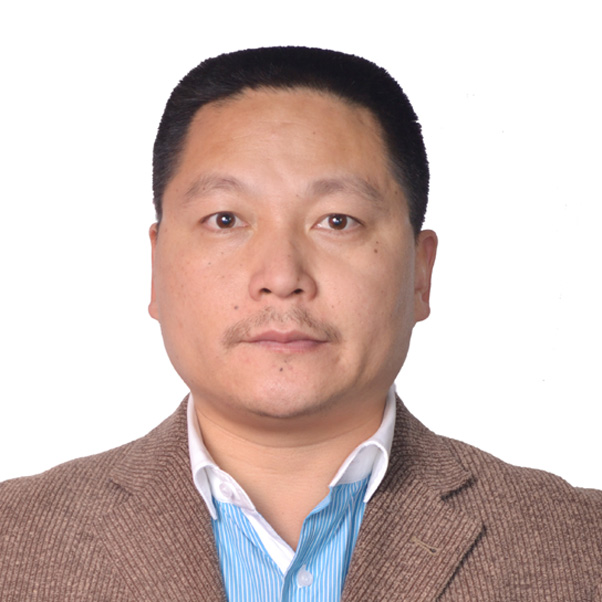
\includegraphics[width=1in,height=1.25in,clip,keepaspectratio]{fig/sanjiang}}]{Sanjiang Li}
received his B.Sc. in mathematics from Shaanxi Normal University in 1996 and his Ph.D. in mathematics from Sichuan University in 2001. He is currently a professor at the Centre for Quantum Software and Information at the University of Technology Sydney (UTS). Prior to joining UTS, he worked in the Department of Computer Science and Technology at Tsinghua University from 2001 to 2008. His primary research interests include knowledge representation, artificial intelligence, and quantum circuit compilation.
\end{IEEEbiography}

\end{document}
